% TrustBand -- Perceptron Hackathon 2026, Round 1 abstract (Problem 10)
% Compile with pdflatex (Overleaf: default settings work). Two pages of text + one diagram page.
% Fill the yellow \ph{...} placeholders (team name/ID, members) before submitting.
\documentclass[10pt,a4paper]{article}

\usepackage[T1]{fontenc}
\usepackage[utf8]{inputenc}
\usepackage[scaled=0.95]{helvet}
\renewcommand{\familydefault}{\sfdefault}
\usepackage[a4paper,top=13mm,bottom=13mm,left=15mm,right=15mm]{geometry}
\usepackage{microtype}
\usepackage{amsmath}
\usepackage{xcolor}
\usepackage{enumitem}
\usepackage{tikz}
\usetikzlibrary{arrows.meta}
\usepackage[hidelinks]{hyperref}

\definecolor{accent}{HTML}{1F4FD1}
\definecolor{muted}{HTML}{5B6170}
\definecolor{alert}{HTML}{B3261E}

\pagestyle{empty}
\setlength{\parindent}{0pt}
\setlength{\parskip}{3pt}
\linespread{1.05}
\setlist{nosep,leftmargin=14pt,itemsep=2pt,topsep=2pt}

\newcommand{\hd}[1]{\par\vspace{6pt}{\color{accent}\bfseries\large #1}\par\vspace{1pt}}
\newcommand{\ph}[1]{\colorbox{yellow!45}{\strut #1}}   % placeholder to fill in

\begin{document}

%-------------------------------------------------------------------- title
{\LARGE\bfseries TrustBand: Trust-Aware Adaptive Conformal Bands for Fusing Manipulable Text with Market Data\par}
\vspace{3pt}
{\color{muted}Problem 10, Theme 6: AI You Can Actually Trust \;$\cdot$\; Team \ph{[Team name / ID]} \;$\cdot$\; Perceptron Hackathon 2026\par}
\vspace{2pt}\hrule height 1pt\vspace{4pt}

%-------------------------------------------------------------------- 1
\hd{1. Problem chosen and why}
A market maker must act on noisy, sometimes hostile information \emph{and know when not to trust its own forecast}. A ``90\%'' band that silently fails in a crash, or is inflated by a bot campaign, is worse than no band.

%-------------------------------------------------------------------- 2
\hd{2. Understanding of the challenge}
We see three cruxes. A quick preliminary check on StockNet (88 US stocks; LightGBM trained on 2014, tested April 2015 to March 2016) confirmed each one and shaped this plan.
\begin{itemize}
  \item \textbf{Market data is not exchangeable.} Split conformal prediction (MAPIE's default) assumes calibration and test errors are interchangeable; regime shifts break this. Its 90\% band covered only \textbf{62\%} of outcomes during the August-2015 crash, while an adaptive version held 85\%.
  \item \textbf{Text's value lies in attention, not sentiment.} Tweet sentiment had $\approx$0 rank correlation with next-day returns, but abnormal tweet-volume spikes preceded $\sim$16--20\% larger moves relative to each stock's own volatility. Text mostly informs \emph{uncertainty}, which is exactly the channel a manipulator can push.
  \item \textbf{Valid is not meaningful.} Coordinated bot posts on 10\% of stock-days widened a naive fusion model's bands by \textbf{23\%} while coverage stayed above 90\%: the bound stayed ``valid'' but carried a spoofed volatility signal. Simple trust-weighting cut this to under 1\%, but bots disguised as real users still added 17\%. Of 119,641 StockNet tweets, 55\% come from automated clients and 40\% are near-duplicates.
\end{itemize}
Two leakage traps also matter: modern LLMs ``know'' post-2015 outcomes (look-ahead bias), and posts made after the 16:00 ET close belong to the next trading day.

%-------------------------------------------------------------------- 3
\hd{3. Proposed approach: TrustBand}
\textbf{Data.} StockNet (88 stocks, 2014--16, raw tweets with account metadata) supplies manipulable social text; FNSPID (15.7M timestamped headlines for S\&P 500 firms, 1999--2023) supplies news; daily OHLCV supplies prices. Each post maps to the first 16:00 ET close after its timestamp; all splits are walk-forward.

\textbf{Text features.} Frozen FinBERT scores each post's sentiment; as a polarity classifier it knows nothing of later prices. Per stock-day we compute sentiment, tweet volume and \emph{abnormal attention} (volume versus the stock's own 20-day average). LLMs (Llama-3 via Groq) only \emph{generate attacks}.

\textbf{Per-post trust scorer.} Tweets: account age, followers, posting rate, posting app, cashtag count, and whether the account has posted about this stock before. News, which has no account data: publisher reputation and how fast the story spreads across outlets. Both: near-identical copies. Hand-written rules give weak labels; LightGBM learns a trust weight $w \in (0,1]$. Text features are recomputed with every post weighted by $w$, and each day gets a trust score $T$.

\textbf{Fusion model.} LightGBM on price features (recent returns, volatility, volume surprise, market moves) plus trust-weighted text: a forecast $\hat{y}$ and an error-size model $\hat{\sigma}(x)$ trained on out-of-fold errors. Low-trust days fall back to a price-only model.

\textbf{Conformal layer.} The band is $\hat{y} \pm q\,\hat{\sigma}(x)$. Adaptive Conformal Inference (Gibbs \& Cand\`es, 2021) updates $q$ daily: widen if more than 10\% of stocks missed, tighten if fewer. High- and low-trust days keep separate $q$'s (Mondrian conformal), so the 90\% guarantee holds \emph{within} suspicious days, not just on average.

%-------------------------------------------------------------------- 4
\hd{4. Minimum viable scope}
\textbf{MV1 (fusion):} FinBERT sentiment, attention and price features feeding LightGBM (prototyped in our preliminary check). \textbf{MV2 (conformal):} MAPIE's off-the-shelf split conformal, plus our adaptive version. \textbf{Demo:} a Streamlit dashboard showing bands per ticker and date, the posts behind them with trust scores, and a live ``inject attack'' slider.

%-------------------------------------------------------------------- 5
\hd{5. Stretch goals}
\textbf{S1, adversarial robustness:} attacker tiers (a) bot flood, (b) LLM-paraphrased unique posts, (c) stealth aged accounts, plus noisy labels flipping 10--30\% of sentiment scores. \textbf{S2, calibration beyond ``present'':} check that 80/90/95\% bands really cover 80/90/95\%, overall and per trust bucket, sector and calm/stress period.

%-------------------------------------------------------------------- 6
\hd{6. Novelty}
\begin{itemize}
  \item Trust controls the conformal layer, so coverage holds within each trust bucket under manipulation.
  \item Manipulation is judged by band inflation and per-group coverage; our check shows overall coverage hides the attack.
  \item The uncertainty channel, not the point forecast, is identified as the main attack surface.
  \item Attackers are adaptive and LLM-generated, not fixed random noise.
\end{itemize}

%-------------------------------------------------------------------- 7
\hd{7. Evaluation plan}
\textbf{Splits:} StockNet train 2014, calibrate Q1-2015, test April 2015 to March 2016 (includes the Aug-2015 and Jan-2016 stress periods); repeated walk-forward on FNSPID 2016--2023 (includes COVID-2020). \textbf{Baselines:} price-only, naive fusion (all posts equal), MAPIE split conformal, adaptive conformal without trust. \textbf{Metrics:} overall, worst-20-day and stress-window coverage; attacked-versus-clean coverage; median width and width inflation; forecast rank correlation. \textbf{Targets:} $\geq$88\% worst-window coverage and $\leq$5\% band inflation under tiers (a)--(b), at $\leq$10\% width cost versus static split.

%-------------------------------------------------------------------- 8
\hd{8. Feasibility and risks}
\textbf{Team.} \ph{[Member 1: data \& NLP]}, \ph{[Member 2: modelling \& conformal]}, \ph{[Member 3: attacks, evaluation \& demo]}. \textbf{Compute:} our preliminary pipeline runs end to end in minutes on an RTX 4050; Kaggle T4$\times$2 handles FinBERT at FNSPID scale.

\textbf{Timeline.} W1 (Nov 10): FNSPID subset and embeddings. W2: trust scorer. W3: trust-weighted fusion, adaptive conformal, trust buckets (midway check). W4: attack tiers and noisy labels. W5: calibration study, dashboard, buffer.

\textbf{Risks.} Text adds little alpha $\rightarrow$ our claim is robust uncertainty, which text demonstrably moves. Stealth attacks evade heuristic trust $\rightarrow$ learned coordination features, ACI as backstop. Stocks crash together, so misses cluster by day $\rightarrow$ day-level updates, and confidence intervals that resample whole days. FNSPID is 5.7\,GB $\rightarrow$ S\&P-100 subset.

%==================================================================== diagram page
\clearpage
\hd{Architecture: TrustBand}
\vspace{6pt}
\begin{center}
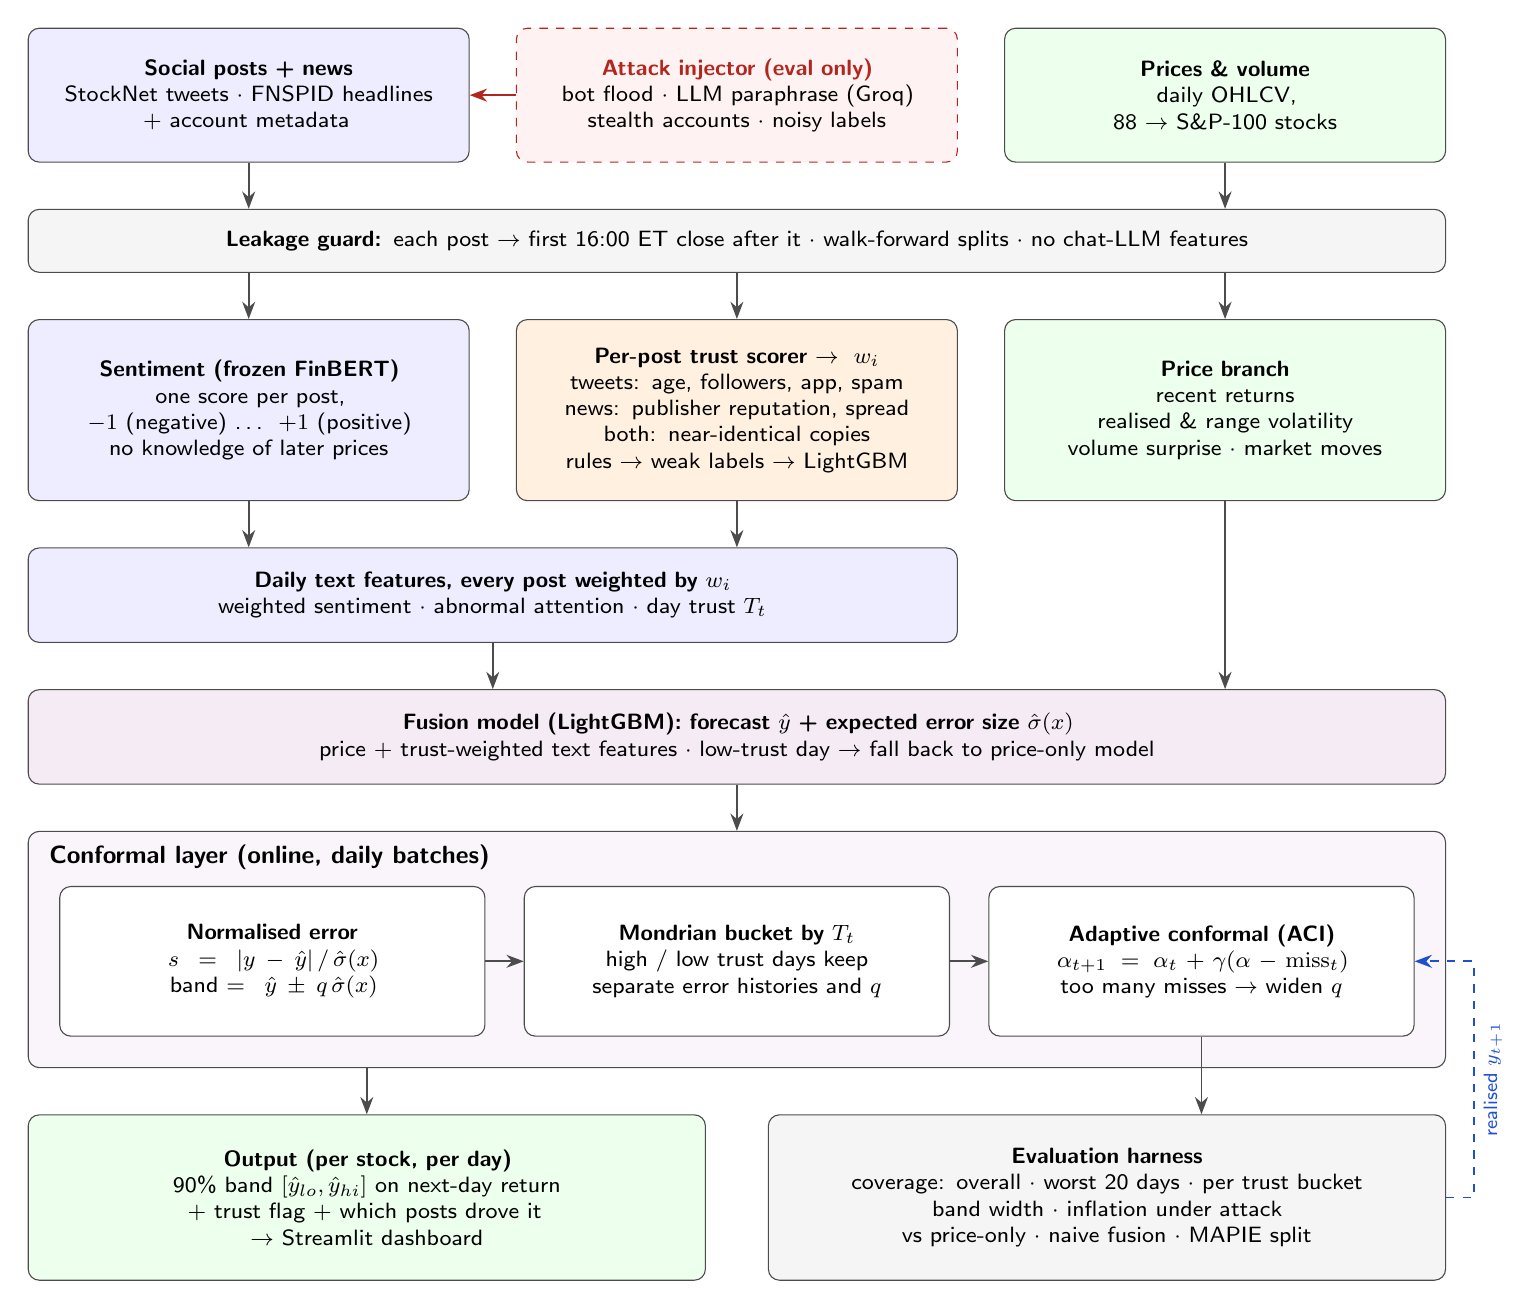
\begin{tikzpicture}[
    x=1cm, y=1cm, font=\footnotesize,
    box/.style={draw=black!70, rounded corners=4pt, anchor=north west, inner sep=0.2cm, align=center},
    arr/.style={-{Stealth[length=2.2mm]}, draw=black!70, line width=0.6pt},
  ]
  % bx{name}{x}{y}{width}{height}{extra style}{content}
  \newcommand{\bx}[7]{\node[box,#6,minimum width=#4cm,minimum height=#5cm,text width={#4cm-0.4cm}] (#1) at (#2,#3) {#7};}

  % row 1: inputs
  \bx{posts}{0}{0}{5.6}{1.7}{fill=blue!7}{\textbf{Social posts + news}\\StockNet tweets $\cdot$ FNSPID headlines\\+ account metadata}
  \bx{attack}{6.2}{0}{5.6}{1.7}{fill=red!5, draw=alert, dashed}{\textbf{\color{alert}Attack injector (eval only)}\\bot flood $\cdot$ LLM paraphrase (Groq)\\stealth accounts $\cdot$ noisy labels}
  \bx{prices}{12.4}{0}{5.6}{1.7}{fill=green!7}{\textbf{Prices \& volume}\\daily OHLCV,\\88 $\rightarrow$ S\&P-100 stocks}
  \draw[arr, draw=alert] (attack.west) -- (posts.east);

  % row 2: leakage guard
  \bx{guard}{0}{-2.3}{18}{0.8}{fill=black!4}{\textbf{Leakage guard:} each post $\rightarrow$ first 16:00 ET close after it $\cdot$ walk-forward splits $\cdot$ no chat-LLM features}
  \draw[arr] (posts.south) -- (posts.south |- guard.north);
  \draw[arr] (prices.south) -- (prices.south |- guard.north);

  % row 3
  \bx{sent}{0}{-3.7}{5.6}{2.3}{fill=blue!7}{\textbf{Sentiment (frozen FinBERT)}\\one score per post,\\$-1$ (negative) \dots{} $+1$ (positive)\\no knowledge of later prices}
  \bx{trust}{6.2}{-3.7}{5.6}{2.3}{fill=orange!12}{\textbf{Per-post trust scorer $\rightarrow w_i$}\\tweets: age, followers, app, spam\\news: publisher reputation, spread\\both: near-identical copies\\rules $\rightarrow$ weak labels $\rightarrow$ LightGBM}
  \bx{price}{12.4}{-3.7}{5.6}{2.3}{fill=green!7}{\textbf{Price branch}\\recent returns\\realised \& range volatility\\volume surprise $\cdot$ market moves}
  \draw[arr] (sent.north |- guard.south) -- (sent.north);
  \draw[arr] (trust.north |- guard.south) -- (trust.north);
  \draw[arr] (price.north |- guard.south) -- (price.north);

  % row 4
  \bx{textf}{0}{-6.6}{11.8}{1.2}{fill=blue!7}{\textbf{Daily text features, every post weighted by $w_i$}\\weighted sentiment $\cdot$ abnormal attention $\cdot$ day trust $T_t$}
  \draw[arr] (sent.south) -- (sent.south |- textf.north);
  \draw[arr] (trust.south) -- (trust.south |- textf.north);

  % row 5
  \bx{fusion}{0}{-8.4}{18}{1.2}{fill=violet!8}{\textbf{Fusion model (LightGBM): forecast $\hat{y}$ + expected error size $\hat{\sigma}(x)$}\\price + trust-weighted text features $\cdot$ low-trust day $\rightarrow$ fall back to price-only model}
  \draw[arr] (textf.south) -- (textf.south |- fusion.north);
  \draw[arr] (price.south) -- (price.south |- fusion.north);

  % row 6: conformal layer (container + three steps)
  \node[box, fill=violet!4, minimum width=18cm, minimum height=3.0cm] (conf) at (0,-10.2) {};
  \node[anchor=north west, font=\small\bfseries] at (0.15,-10.25) {Conformal layer (online, daily batches)};
  \bx{score}{0.4}{-10.9}{5.4}{1.9}{fill=white}{\textbf{Normalised error}\\$s = |y-\hat{y}|\,/\,\hat{\sigma}(x)$\\band $=\hat{y} \pm q\,\hat{\sigma}(x)$}
  \bx{mond}{6.3}{-10.9}{5.4}{1.9}{fill=white}{\textbf{Mondrian bucket by $T_t$}\\high / low trust days keep\\separate error histories and $q$}
  \bx{aci}{12.2}{-10.9}{5.4}{1.9}{fill=white}{\textbf{Adaptive conformal (ACI)}\\$\alpha_{t+1} = \alpha_t + \gamma(\alpha - \mathrm{miss}_t)$\\too many misses $\rightarrow$ widen $q$}
  \draw[arr] (score.east) -- (mond.west);
  \draw[arr] (mond.east) -- (aci.west);
  \draw[arr] (fusion.south) -- (fusion.south |- conf.north);

  % row 7
  \bx{out}{0}{-13.8}{8.6}{2.1}{fill=green!7}{\textbf{Output (per stock, per day)}\\90\% band $[\hat{y}_{lo}, \hat{y}_{hi}]$ on next-day return\\+ trust flag + which posts drove it\\$\rightarrow$ Streamlit dashboard}
  \bx{eval}{9.4}{-13.8}{8.6}{2.1}{fill=black!4}{\textbf{Evaluation harness}\\coverage: overall $\cdot$ worst 20 days $\cdot$ per trust bucket\\band width $\cdot$ inflation under attack\\vs price-only $\cdot$ naive fusion $\cdot$ MAPIE split}
  \draw[arr] (out.north |- conf.south) -- (out.north);
  \draw[arr] (aci.south) -- (aci.south |- eval.north);
  % feedback: realised returns update the online conformal step
  \draw[arr, draw=accent, dashed] (eval.east) -- ++(0.35,0) |- (aci.east)
        node[pos=0.25, font=\scriptsize, text=accent, rotate=90, anchor=north] {realised $y_{t+1}$};
\end{tikzpicture}
\end{center}

\vspace{4pt}
{\small\color{muted}Blue: text lane $\cdot$ amber: trust $\cdot$ green: price lane $\cdot$ purple: fusion and conformal layer $\cdot$ dashed red: attack injection (evaluation only) $\cdot$ dashed blue: realised returns feed back into the daily conformal update.\par}

\end{document}
